\section{Experiment}
In diesem Kapitel werden die Sicherheitsgefahren und -risiken von IoT-Geräten demonstriert. 
Dafür wird eine Raspberry Pi-Sicherheitskamera mithilfe der Open-Source-Bibliothek \textit{pi-aREST} 
entwickelt. Die Sicherheitskamera sendet mithilfe von \textit{pi-aREST} in einem festgelegten 
Zeitintervall ein Bild, des überwachten Bereichs, an ein externes System. Die Entscheidung \textit{pi-aREST} 
als Bibliothek für die Entwicklung des IoT-Gerätes zu verwenden, hatte mehrere Gründe. 
Zum einen ist der Quellcode Open-Source, wodurch potentielle Sicherheitsrisiken gezielter festgestellt
und untersucht werden können. Außerdem bietet der Entwickler der Bibliothek einen eigenen Überwachungs 
und Kontroll-Service, für die mit der Bibliothek entwickelten IoT-Geräte, an. Wodurch die Untersuchung
der möglichen Sicherheitsprobleme anhand von realisitischen Szenarien demonstriert werden kann.  \\

Erwähne das für Kamera und das im speziellen für IOT
Dafür wird eine Raspberry -> Dafür wurde eine ... (alles in Vergangenheit)

\begin{figure}[h]
  \centering
  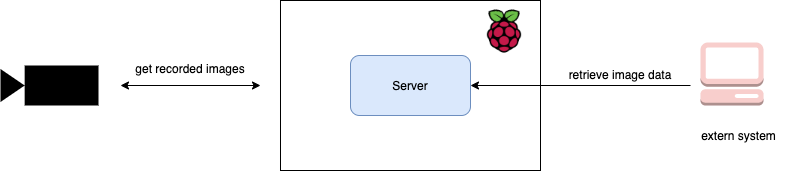
\includegraphics[width=145mm]{images/raspberrypi.png}
  \caption{Sicherheitskamera-Architektur}
  \label{fig:arch-raspberrypi}
\end{figure}


\subsection{pi-aREST}
\textit{pi-aREST} ist eine Bibliothek für die JavaScript-Laufzeitumgebung \textit{Node.js}, welche mithilfe
des Package-Managers \textit{npm} in eine Node-Anwendung importiert werden kann. Durch das Einbinden
von \textit{pi-aREST} in eine eigene Node-Anwendung werden Schnittstellen zur Kommunikation mit anderen
Systemem und Geräten geöffnet. Der Datenaustausch erfolgt dabei mithilfe der Protokolle \textit{HTTP} 
und \textit{MQTT} und kann sowohl in lokalen Netzwerken, als auch im Internet stattfinden.

\subsubsection{HTTP-Server}
Nachdem Ausführen der Node-Anwendung mit der importierten Bibliothek, startet \textit{pi-aREST} einen 
\textit{express} HTTP-Server auf dem IoT-Gerät zum bereitstellen einer REST-API. Die API besitzt
verschiedene Endpunkte, welche entweder innerhalb des Netzwerkes oder aus dem Internet aufgerufen werden
können. 

Tabelle Server

\subsubsection{MQTT-Client}
Message Queuing Telemetry Transport (MQTT) ist ein Open-Source Kommunikationsprotokoll auf der
Anwendungsebene. Das Protokoll zeichnet sich durch ressourcensparende Datenpakete mit einem 
geringen Overhead aus, wodurch es bspw. oftmals in der Kommunikation zwischen IoT-Geräten (M2M) 
eingesetzt wird. Das Protokoll basiert auf der Publish/Subscribe-Architektur, so nehmen Clients
die Rollen eines Publisher (Sender) oder Subscriber (Empfänger) ein. Die Hauptkomponente, welche
die Client miteinander verbindet und die Datenbewegungen steuert, ist der Broker.  Mit diesem
verbinden sich sowohl Publisher, als auch die Subscriber. Sendet ein Publisher Daten an den Broker,
werden diese von dem Broker an die Subscriber weitergeleitet. 

Beim Ausführen der Node-Anwendung mit \textit{pi-aREST} verbindet sich das IoT-Gerät als Publisher-Client
mit einem MQTT-Broker über den Port 1883. Die Broker-Adresse wird von der Node-Anwendung vorgegeben,
\textit{pi-aREST} sendet daraufhin die Verbindungsanfrage an den Broker. Das IoT-Gerät sendet nach dem 
erfolgreichen Verbindungsaufbau in einem regelmäßigen Zeitintervall, im Falle des Experiementes die 
Überwachungsbilder, an den Broker.



GRAFIK


